\documentclass{scrartcl}

\usepackage[utf8]{inputenc}


% zus�tzliche mathematische Symbole, AMS=American Mathematical Society 
\usepackage{amssymb}
\usepackage{amsmath}
\usepackage{amsthm}
\usepackage{bbm}
\usepackage{color}
\usepackage{listings}
\usepackage{pdfpages}
\usepackage{csquotes}

% f�rs Einbinden von Graphiken
\usepackage{graphicx}

% f�r Namen etc. in Kopf- oder Fu�zeile
\usepackage{fancyhdr}
\usepackage{tikz}
\usetikzlibrary{arrows, automata}

% erlaubt benutzerdefinierte Kopfzeilen 
\pagestyle{fancy}

% Definition der Kopfzeile
\lhead{
\begin{tabular}{lll}
Johannes Kalmbach &  &   \\
\end{tabular}
}
\chead{}
\rhead{\today{}}
\lfoot{}
\cfoot{Seite \thepage}
\rfoot{} 

\begin{document}

\section*{Deep Learning Lab, Report for Submission 1}
\subsection*{Implementation Status}
In general my submissions contains all the requested features. It additionally contains the following bonus features:
\begin{itemize}
	\item Random dropout of weights and biases
	\item L2-Regularization (I did not add the penalty term to the actual loss function but only used the regularization when computing the gradients. This is possible because the penalty term of a given parameter only affects the gradient of this parameter).
	\item RMSprop Optimizer. This needs an additional parameter for each weight (the average squared history) and thus increases the memory usage.
\end{itemize}
Given the task of the exercise sheet my submission currently has the following limitations:
\begin{itemize}
	\item There currently are no stopping criteria other than \enquote{train for the given number of epochs}. I found out during my experiments that this feature could be useful to avoid unnecessary epochs that are expensive in bigger nets.
	\item The SGD optimizer currently only supports a constant learning rate and no more advanced learning rate schedule techniques. I mostly used my RMSprop optimizer for the experiments which to my understanding worked well.
\end{itemize}
I hope that my implemented bonus features will make up for those missing features.
\subsection*{Experiments and Results}
After playing around a bit initially I limited myself to the following tasks:
\begin{itemize}
	\item Find a network that is powerful enough to represent the connection between the training data and the output
	\item See how much this network overfits and apply regularization techniques to keep the training and the validation loss connected.
\end{itemize}
For most of the experiments I used the \textbf{RMSprop} optimizer with a forgetting parameter of $0.9$ and a learning rate of $0.001$. These are according to literature the default parameters for this optimizer and I found them to lead to fast convergence also in my application. \\
I found that a net with 2 hidden layers of 800 neurons each was powerful enough to learn the training set almost completely. The training and validation loss of this experiment can be seen in figure \ref{fig:noDropout}
\begin{figure}
	\centering
	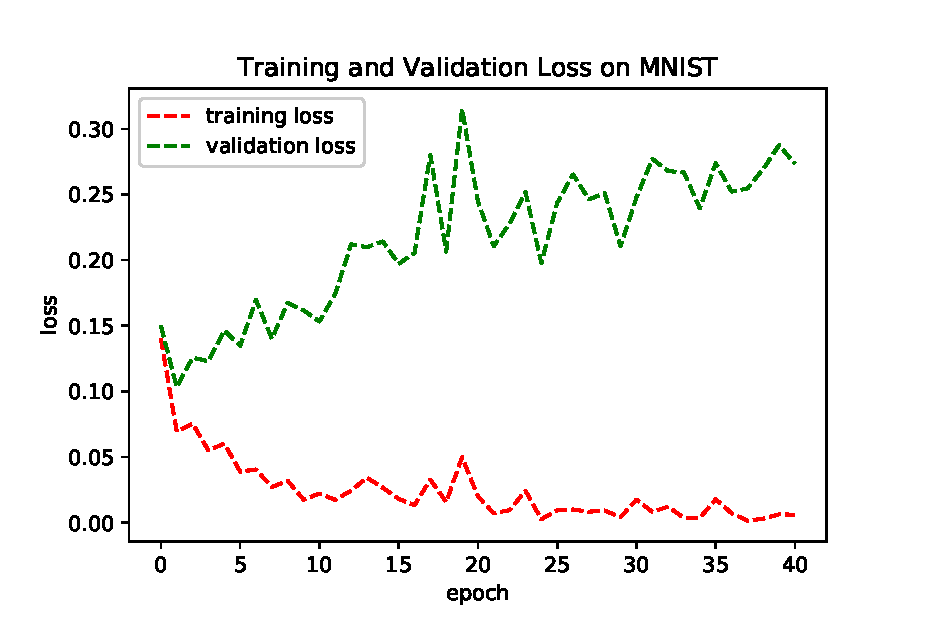
\includegraphics[scale=0.7]{no_dropout.eps}
	\caption{2 hidden layers with 800 neurons each, ReLU activation, no regularization, 40 epochs}
	\label{fig:noDropout}
\end{figure}
In this figure we can observe the following:
\begin{itemize}
	\item This model clearly overfits, as the training loss goes to zero while the validation loss increases at first.
	\item The overfitting only starts at the third epoch. This means that stopping the training earlier can reduce overfitting.
\end{itemize}
As a next step I applied a dropout of 50\% and got the results from figure \ref{fig:withDropout}. 
\begin{figure}
	\centering
	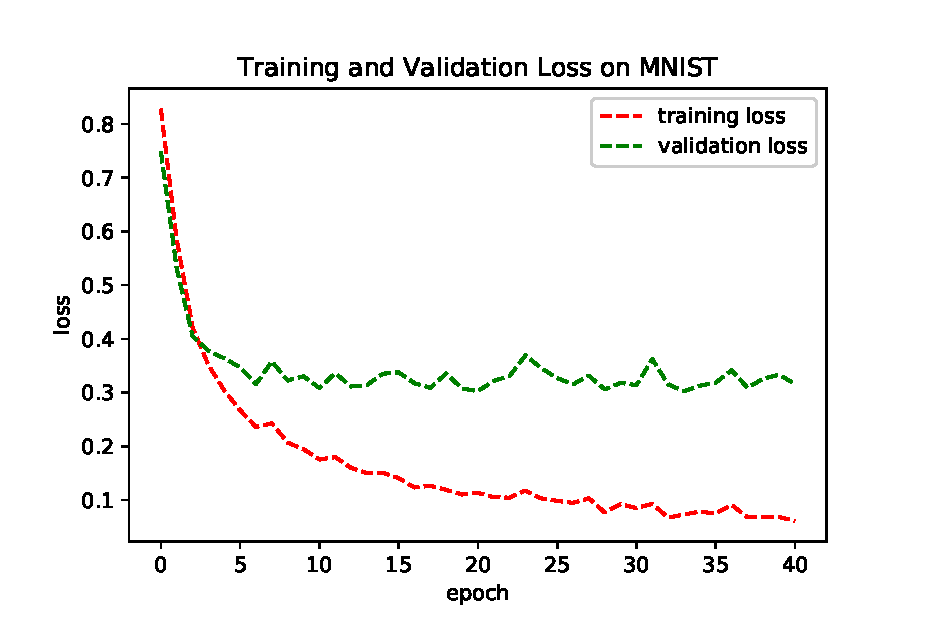
\includegraphics[scale=0.7]{with_dropout.eps}
	\caption{2 hidden layers with 800 neurons each, ReLU activation, dropout factor 0.5, 40 epochs}
	\label{fig:withDropout}
\end{figure}
We see that the absolute loss values stay worse than in the unregularized case and that we still have overfitting. \\
I also made the following (strange) observation:
My training routine also plots the validation error and not only the loss and I found out that those two are not really closely coupled.
Although the validation loss slightly increases in figure \ref{fig:noDropout}, the error on the validation set keeps going down. I am not sure if this is a typical behavior of the softmax cross entropy loss or if there might be something wrong in my code. \\
For my final observations I merged the training and validation set and compared against the test data. The losses of this run can be seen in figure \ref{fig:finalResults}.
\begin{figure}
	\centering
	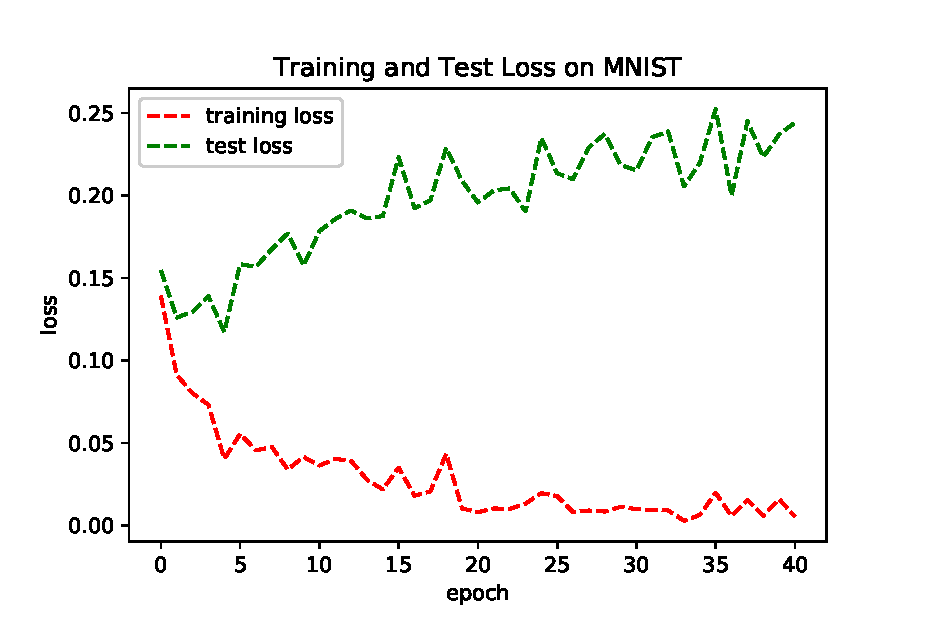
\includegraphics[scale=0.7]{test_result.eps}
	\caption{2 hidden layers with 800 neurons each, ReLU activation, no regularization, 40 epochs}
	\label{fig:finalResults}
\end{figure}
What can be observed in this figure is that the two loss functions are still connected (peaks in the training loss are also peaks in the validation loss) which could be a sign for the overfitting not being too bad. \\
The final result on the test set yielded an error rate of \textbf{1.73\%} which I consider to be pretty decent for my first tries with deep learning in practice.
\subsection*{Feedback}
I am attending the \enquote{Foundations of Deep Learning} lecture in parallel where we also have to implement a feed forward network this week. The stubs that are provided differ in several aspects. While the one provided for this lab is simpler (less arguments, less abstract base classes) it is harder to implement extra features. While I found it pretty straightforward to code the basic features I sometimes found it hard to include extra features like regularization or more optimizers in a architecturally clean way. For these aspects the stub from the Deep Learning lecture is probably a bit better. There they try to mimic the API of an existing framework (pytorch in their case) which will be used later in the course. I am not sure how long we will work with our own implementation in this lab and if or when we will start using existing framework but maybe this point could be taken into consideration for upcoming versions of this course.

But overall I really liked this sheet and was really pleased when the gradient checks worked for the first time and when I was able to get error rates below 2\%.


\end{document}


